\documentclass[11pt]{article}
\usepackage{graphicx}
\usepackage{float}
\usepackage{amsmath}
\usepackage{amsfonts}
\usepackage[brazilian]{babel}
\usepackage[utf8]{inputenc}
\usepackage[backend=biber]{biblatex}
\usepackage{csquotes}
%\usepackage{docmute}
\usepackage{array}
\ifdefined\multicol
	\usepackage{multicol}
	\usepackage{geometry}
\fi
\usepackage[T1]{fontenc}

\addbibresource{plano_de_pesquisa.bib}

\newcommand{\fromeng}[1]{\footnote{do inglês: \textit{#1}}}
\newcommand{\tit}[1]{\textit{#1}}
\newcommand{\tbf}[1]{\textbf{#1}}
\newcommand{\ttt}[1]{\texttt{#1}}

\newcolumntype{C}[1]{>{\centering\let\newline\\\arraybackslash\hspace{0pt}}m{#1}}

\begin{document}

\begin{titlepage}
	\centering
	{\scshape\Large Projeto de pesquisa\par}
	\vspace{1.5cm}
	{\huge\bfseries Processos atencionais e aprendizado de máquina 
		para sistemas robóticos\par}
	\vspace{1cm}
	{\itshape Aluno: Erik de Godoy Perillo\par}
	{\itshape Orientadora: Profa. Dra. Esther Luna Colombini\par}
	\vspace{0.5cm}
	\begin{abstract}
		Entender o ambiente ao seu redor é uma tarefa fundamental para 
		o desafio de se obter máquinas autônomas que interagem com o 
		mundo de forma semelhante à nossa.
		No entanto, a alta dimensionalidade dos dados captados por sensores 
		usados para este fim é em geral problemática, muitas vezes havendo
		redundância e irrelevância de informação. 
		Nos seres humanos este filtro sensorial é realizado pela Atenção.
		Neste contexto, este projeto propõe a aplicação de técnicas de 
		aprendizado de máquina sobre informações sensoriais previamente 
		processadas por processos atencionais em uma tarefa de navegação 
		autônoma.  
		Adicionalmente, planeja-se implementar uma estrutura que permita o 
		uso das técnicas propostas para projetos robóticos em geral que 
		utilizem GPUs embarcadas.
	\end{abstract}
	\vfill
	Universidade Estadual de Campinas 
	\vfill
	{\large \today\par}
\end{titlepage}

\newpage

\section{Introdução}
\paragraph{}
Máquinas capazes de realizar tarefas complexas, perigosas ou maçantes são
objeto de interesse e desejo do ser humano há tempos. 
Robôs industriais já dominam os mais variados setores de produção. 
Não apenas parados em linhas de montagem, sistemas atuais podem locomover-se
em regiões uniformes e previsíveis -- como galpões de estoques -- trabalhando
vinte e quatro horas por dia~\cite{warehouse}.
Um desafio ainda em aberto, entretanto, é a concepção de robôs que lidam com 
o imprevisível, reagindo de forma apropriada às mais diversas situações 
e ambientes do mundo real. 

Sistemas que interagem com o ambiente, objetos e pessoas 
com uma variedade de maneiras semelhante à nossa têm o potencial de ser 
benéficos para a sociedade. 
%Esse tipo de robô tem sido tendência ...
Entretanto, diversos são os desafios associados ao processo de concepção de 
máquinas gerais desse tipo. 
Um deles, certamente, é a compreensão do ambiente. 
Entender o que lhe cerca é fundamental para uma interação complexa com o resto
do mundo. 

Ter ciência de sua relação com outros objetos e 
as possíveis interações com cada um deles é essencial para a navegação 
de robôs por casas, ruas e até mesmo locais onde a presença de humanos seria 
impossível ou indesejável.
Essa é uma das tarefas principais que máquinas como carros autônomos, 
robôs de serviço \cite{ifr} e de resgate devem cumprir bem. 
Para tal, os robôs são dotados de sensores como câmeras~\cite{vision} e 
LIDAR~\cite{car} têm sido usadas com sucesso para identificação e 
classificação de entidades em um ambiente com o qual o robô interage. 

\subsection{Motivação}
\paragraph{}
Um problema de sensores usados para tarefas mais complexas de navegação
em geral -- como câmera, LIDAR e outros sensores --
é que o volume de dados a ser processado podem ser demasiadamente grande. 
Para um robô que interage continuamente com o ambiente, é improvável que em 
todos os instantes  toda informação proveniente de seus sensores seja 
processada ou mesmo necessária. 
Lidar com todo o conjunto de dados para depois determinar qual parte é 
relevante pode ser uma tarefa  computacionalmente custosa. 
Isso é especialmente crítico para sistemas robóticos que precisam de respostas
rápidas para interagir com o ambiente em que estão inseridos. 

Além disso, o \tit{hardware} utilizado em robôs autônomos tem sido, por muitos 
anos, limitado às restrições geradas pela necessidade de embarcá-lo em sistemas 
compactos. 
Entretanto, avanços recentes têm mudado isso. 
Além do aumento da eficiência e diminuição do tamanho de CPUs impulsionado pelo 
mercado \tit{mobile}, esforços têm sido feitos para a concepção de computadores 
com processadores gráficos (GPUs) embarcados, que permitem o tratamento 
eficiente de dados naturalmente característicos dos sensores empregados.  
A \tit{NVIDIA} lançou recentemente os modelos 
\tit{Jetson TK1} e \tit{Jetson TX1}~\cite{jetson}, que são sistemas 
computacionais completos com GPUs poderosas e energeticamente eficientes, 
desenvolvidos especialmente para serem embarcados em projetos móveis.
O uso de GPUs em robótica abre a possibilidade do uso de técnicas mais 
sofisticadas e computacionalmente caras que até então não podiam ser exploradas.
Sua natureza paralela permite um grande benefício de operações que podem ser
divididas em subproblemas e realizados ao mesmo tempo. 
Esse é o caso de diversas tarefas realizadas no processamento de sinais e por 
técnicas de aprendizado de máquina~\cite{gpu}, por exemplo. 

\subsection{Processos atencionais e aprendizado de máquina}
\paragraph{}
O fato de sensores darem uma quantidade muito grande de informação que nem 
sempre é necessária motiva uma abordagem inspirada no ser humano.
Não damos foco a todas as conversas que escutamos ou em tudo que vemos, mas sim 
apenas na parte que nos convém ou cuja natureza é extremamente atrativa. 
Nos seres humanos este filtro sensorial é realizado pela 
Atenção~\cite{Dux_Marois_2009}. 
Técnicas que fazem uso de processos atencionais têm sido usadas para a 
segmentação de áreas de relevância na percepção e entendimento do 
ambiente com sucesso~\cite{bio}~\cite{esther}.
Com essas abordagens, pode-se filtrar dados irrelevantes ou
redundantes, dando prioridade e foco a elementos relavantes do ambiente, 
aumentando consideravelmente a eficiência computacional dessas técnicas. 

Porém, não só o foco é necessário. Em ambientes dos mais variados é preciso, 
além de identificar, classificar entidades a fim de interagir com elas de forma
apropriada. 
O aprendizado de máquina tem sido uma área de grande sucesso nessa tarefa.
Diversas técnicas podem ser utilizadas, como \tit{SVMs}~\cite{svm} 
e redes neurais~\cite{nn} a fim de se classificar entidades em geral com 
alta taxa de acertos. 

Neste sentido, este projeto busca uma associação dessas técnicas: o uso dos 
processos atencionais em um estágio inicial de processamento pode atuar como um 
filtro na informação, passando adiante o que é relevante para o estágio de
classificação, a ser suportado por técnicas de aprendizado de máquina. 
Espera-se que tal abordagem possibilite uma percepção eficiente para sistemas 
autônomos o que permitiria a realização de tarefas mais sofisticadas, trazendo 
benefícios objetivos para a área da percepção em robótica.

\section{Objetivos}
\paragraph{}
O objetivo geral deste trabalho envolve a aplicação de técnicas de aprendizado 
de máquina sobre informações sensoriais previamente processadas pelo modelo 
atencional proposto por em \cite{esther} em uma tarefa de navegação autônoma.  

Mais especificamente, objetivamos:
\begin{itemize}
	\item Obter técnicas que permitam o entendimento de ambientes
		diversos para a navegação de sistemas robóticos autônomos por meio 
		do uso de processos atencionais e aprendizado de máquina;
	\item Avaliar a efetividade e eficiência da abordagem proposta
		comparado a outras técnicas utilizadas atualmente;
	\item Construir uma plataforma para uso em GPUs embarcadas com 
		ferramentas que permitam o uso das técnicas desenvolvidas para
		aplicações variadas de robótica.
\end{itemize}

\section{Materiais e Métodos}

Para atendimento dos objetivos propostos, serão realizadas as seguintes etapas:

\begin{itemize}
	\item FASE  1:  Revisão  bibliográfica. Nesta etapa, será realizada a 
		revisão bibliográfica:  a) do  modelo  atencional \cite{esther}, 
		buscando quais adequações serão necessárias para o projeto em questão, 
		e b) das técnicas de Aprendizado de Máquina mais 
		apropriadas para a tarefa;
	\item FASE  2: Preparação do ambiente computacional. 
		Nessa fase, o ambiente para construção do sistema será preparado 
		(configuração do ambiente, instalação de bibliotecas e softwares, 
		instalação de pacotes gráficos, configurações, etc); 
	\item FASE  3:  Modelagem e implementação de processos atencionais.  
		Nessa  etapa  será proposta a base do sistema  atencional e testes 
		preliminares serão realizados;
	\item FASE  4:  Modelagem e implementação da técnica de aprendizado de 
		máquina.  
		Nessa  fase  a  técnica escolhida na FASE 1 será implementada e 
		testes preliminares serão realizados; 
	\item FASE  5:  Integração dos sistemas.
		Nessa fase será realizada a integração do sistema atencional à técnica 
		de aprendizado de máquina;
	\item FASE  6:  Testes comparativos. 
		Nessa fase serão realizados testes  e  ensaios  com  o  agente  
		robótico executando o sistema integrado;
	\item FASE  7:  Construção de plataforma para GPU. 
		Nesta etapa o sistema proposto será adequado para ser executado na GPU;
	\item FASE  8:  Relatório final. 
		Redação do relatório final.
\end{itemize}

\subsection{Ambiente}
\paragraph{}
O desafio \tit{Trekking}~\cite{trekking_regras} é uma categoria da série de 
competições de robótica realizada pela \tit{Robocore}~\cite{robocore}. 
Nesta categoria, o robô deve completar um percurso em 
um campo de futebol passando por diversas bases em uma ordem pré-definida.
Em uma certa região do campo, há obstáculos dos quais o robô deve desviar 
(Figura \ref{fig:ambiente}).  
O percurso deve ser feito no menor tempo possível.

\begin{figure}[hbt]
\begin{center}
		\begin{tabular} {cc}
		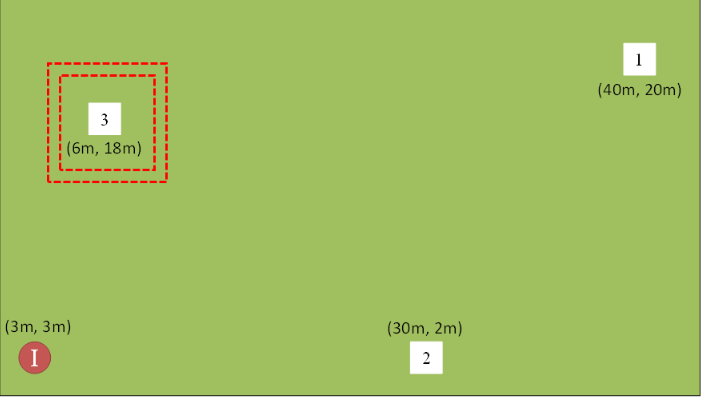
\includegraphics[width=0.49\textwidth]{imgs/trekking_campo.png} &
		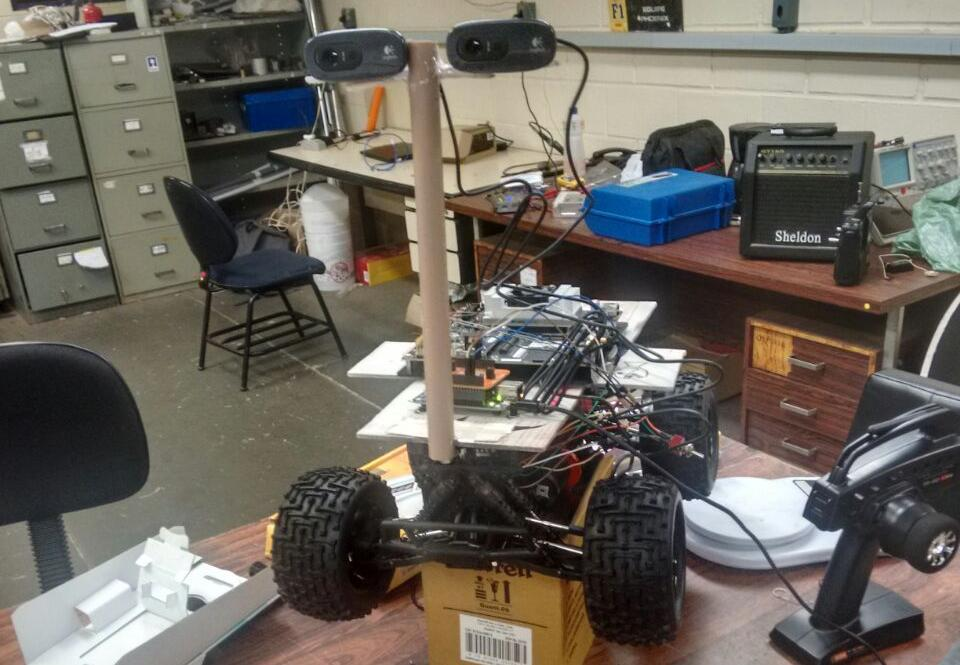
\includegraphics[width=0.4\textwidth]{imgs/piranha.jpg} \\
		(a) & (b) \\
		\end{tabular}
\end{center}
\caption{a) O ambiente de locomoção do robô na categoria Trekking 
	b) Robô utilizado na competição.}
\label{fig:ambiente}
\end{figure}

A \emph{Equipe Phoenix de Robótica da Unicamp}~\cite{phoenix} 
é formada por estudantes de graduação de diversos cursos de 
Engenharia e Computação da Universidade Estadual de Campinas. 
A equipe desenvolve atualmente um robô para participar na categoria 
\tit{Trekking}, apresentado na Figura \ref{fig:ambiente} b).
O robô consiste em um carro elétrico com tração nas quatro rodas e 
locomoção por motores \tit{brushless}.
O motor é controlado por meio de um conjunto da \tit{NXP} composto da placa
\ttt{FRDM-K64F} e da placa \ttt{FRDM-STBC-AGM01}~\cite{nxp}, que contém 
diversos sensores inerciais como magnetômetro, giroscópio e acelerômetro.
Há também um kit de desenvolvimento com GPU embarcada \tit{NVIDIA Jetson TX1}. 
A \tit{Jetson TX1} possui um processador \tit{ARM Quad-Core Cortex-A57},
4GB de memória \tit{RAM} e uma GPU \tit{NVIDIA Maxwell} com 256 núcleos de
processamento~\cite{tx1}. 
Seu sistema operacional é o Ubuntu com \tit{kernel Linux}.
Duas câmeras \tit{Logitech C270} são os sensores
principais usados pela \tit{Jetson TX1} para a ambientação do robô no campo.

A pesquisa usará este robô como caso de uso para
avaliação da abordagem a ser desenvolvida, com o uso da \tit{Jetson TX1} 
como plataforma para implementação das técnicas.
O robô usa a câmera como principal sensor, podendo contar com o apoio de sensores auxiliares.

Na tarefa de navegação proposta o robô deverá reconhecer o terreno no qual pode mover-se, os obstáculos do
qual deve desviar e bases nas quais deve chegar.

\subsection{Avaliação da abordagem proposta}
\paragraph{}
Para efeitos de avaliação, serão comparadas os cenários onde: 
\begin{enumerate}
	\item Uma abordagem específica é utilizada.  
		Um simples \tit{threshold} de cor pode ser capaz de identificar objetos
		imagem e classificá-los dado que diferentes classes de objetos têm
		diferentes cores.
	\item Aprendizado de máquina puro para reconhecimento de objetos.
		Nessa abordagem, será dado foco igual a toda a informação. 
		Assim, todo o conjunto deverá ser analisado pelos algoritmos de 
		classificação.
	\item Processos atencionais são utilizados em um estágio anterior ao de 
		classificação com aprendizado de máquina, com a intenção de selecionar
		subconjuntos de toda informação dada pelo sensor que tenham maior 
		relevância para serem analizados no estágio de classificação.
\end{enumerate}

Com essa comparação, espera-se avaliar cada técnica pelos seguintes critérios:
\begin{itemize}
	\item Desempenho: o custo computacional da técnica.
	\item Eficiência: quão corretamente a técnica identifica e classifica
		as entidades de interesse.
	\item Generalidade: possibilidade da técnica ser utilizadas em outros 
		cenários.
\end{itemize}

\subsection{Construção de plataforma para navegação usando GPUs}
\paragraph{}
Com as técnicas obtidas pelo projeto, espera-se construir uma plataforma
de uso geral para robôs autônomos que usem GPUs embarcadas.
\tit{frameworks} de aprendizado de máquina serão estudados para se decidir
quais usar. 
Toda biblioteca será escolhida de forma que se possa utilizar o processamento
da GPU. O sistema será construído em \tit{C++} e \tit{Python}.

\section{Cronograma}
\paragraph{}
\begin{table}[H]
\centering
\setlength{\tabcolsep}{.16667em}
\begin{tabular}{|C{3cm}|c|c|c|c|c|c|c|c|c|c|c|c|}
	\hline
	Tarefa/mês & Jul & Ago & Set & Out & Nov & Dez & Jan & Fev & Mar & Abr 
		& Mai & Jun \\
	\hline
	FASE 1 & x & x & & & & & & & & & &\\
	\hline
	FASE 2 & x & x & x & & & & & & & & & \\
	\hline
	FASE 3 & & x & x & x & x & & & & & & &  \\
	\hline
	FASE 4 & & x & x & x & x & x & & & & & &  \\
	\hline
	FASE 5 & & & & & x & x & x & x & x & & & \\
	\hline
	FASE 6 & & & & & & & x & x & x & & & \\
	\hline
	FASE 7 & & & & & & & & & & x & x & \\
	\hline
	FASE 8 & & & & & & & & & & & x & x \\
	\hline
\end{tabular}
\end{table}

\printbibliography

\end{document}
